
\documentclass[12pt,journal,compsoc]{IEEEtran}
\usepackage{array}
\usepackage{bytefield}
\usepackage{graphicx}
\usepackage{listings}
\usepackage{slashbox}
\usepackage{tikz}
\lstset{
frame=tb,
language=C,
aboveskip=3mm,
belowskip=3mm,
showstringspaces=false,
columns=flexible,
basicstyle={\small\ttfamily},
numbers=none,
breaklines=true,
breakatwhitespace=true,
tabsize=3
}
\hyphenation{op-tical net-works semi-conduc-tor}
\newcounter{mcount}
\setcounter{mcount}{0}
\begin{document}
\title{Chat System}
\author{David Gong, Stephen Hamilton}% <-this % stops a space
\date{Sunday, September 21, 2014}
\IEEEtitleabstractindextext{%
\begin{abstract}
Our goal is to develop a distributed chat server client system that is fault tolerant. 
\end{abstract}
}
\maketitle
\section{Introduction}
\IEEEPARstart{T}{his} system will be composed of a client and a server.  Servers will communicate through spread and utilize multicast with agreed ordering.  
\section{Design}
\subsection{Assumptions}
Below are our assumptions.
\begin{itemize}
\item A user is uniquely identified by their screen name.
\item 
\end{itemize}
\subsection{Chat Message Packet}
\begin{lstlisting}
// Structure of chat packet.
int type;//Type of packet 0 for message, 1 for like
int sequence; //Sequence of message given to the server
int server_id; //Server id that the message was created on.
char name[25]; //Text name of user
char group[25]; //Text name of chat room
char text[80]; //Text of chat message
int like_sequence; //Integer of sequence number of message liked\
int resend; //Set to 1 if the message is a resend for other servers
\end{lstlisting}
The message packet is utilized for both chat messages and likes created by a user.  The message packet will be saved to disk when received from spread, and the sequence number will be assigned upon receiving it from spread (it is null initially).

\subsection{Server State Machine}
\begin{center}
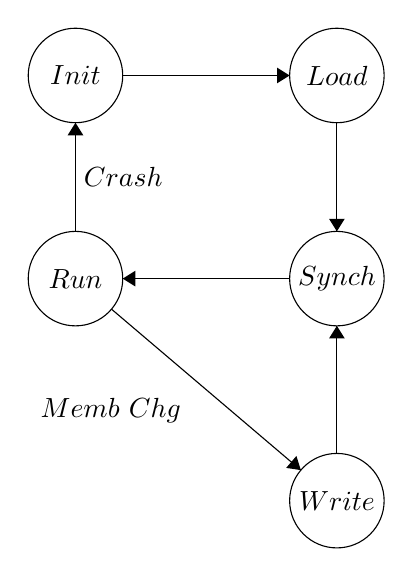
\begin{tikzpicture}[scale=0.2]
\tikzstyle{every node}+=[inner sep=0pt]
\draw [black] (3.3,-3.5) circle (3);
\draw (3.3,-3.5) node {$Init$};
\draw [black] (19.9,-3.5) circle (3);
\draw (19.9,-3.5) node {$Load$};
\draw [black] (19.9,-16.4) circle (3);
\draw (19.9,-16.4) node {$Synch$};
\draw [black] (3.3,-16.4) circle (3);
\draw (3.3,-16.4) node {$Run$};
\draw [black] (19.9,-30.5) circle (3);
\draw (19.9,-30.5) node {$Write$};
\draw [black] (6.3,-3.5) -- (16.9,-3.5);
\fill [black] (16.9,-3.5) -- (16.1,-3) -- (16.1,-4);
\draw [black] (19.9,-6.5) -- (19.9,-13.4);
\fill [black] (19.9,-13.4) -- (20.4,-12.6) -- (19.4,-12.6);
\draw [black] (3.3,-13.4) -- (3.3,-6.5);
\fill [black] (3.3,-6.5) -- (2.8,-7.3) -- (3.8,-7.3);
\draw (3.8,-9.95) node [right] {$Crash$};
\draw [black] (16.9,-16.4) -- (6.3,-16.4);
\fill [black] (6.3,-16.4) -- (7.1,-16.9) -- (7.1,-15.9);
\draw [black] (5.59,-18.34) -- (17.61,-28.56);
\fill [black] (17.61,-28.56) -- (17.33,-27.66) -- (16.68,-28.42);
\draw (5.54,-23.94) node [below] {$Memb\mbox{ }Chg$};
\draw [black] (19.9,-27.5) -- (19.9,-19.4);
\fill [black] (19.9,-19.4) -- (19.4,-20.2) -- (20.4,-20.2);
\end{tikzpicture}
\end{center}
\subsection{Data Structure}
We will utilize a linked list to store the chat messages.  This will give us the ability to store a dyanmic amount of messages, and discard them once all servers are synced.  There will be one array containing an index for each machine, and will have the linked list containing the messages which are stored in the struct defined by our chat message packet.
\subsection{Design}
We plan to have each server save every message it receives from a client to disk.  We will also have a file that contains messages from all servers that will be written every time there is a membership change.  Sequence numbers will be assigned to each message when it is received from Spread, and a client will not see their message until the server that put it into spread received the message and has a sequence number assigned to it.  Servers will continue to run during a partition.  When a partition merges, the partition that contained the lowest numbered server will have priority to send.  Each server will send its vector containing the highest number sequence from each server.  Each server will resend the messages from the lowest heard sequence for their server.  The ordering will be maintained by the sequence number, and further ordering will be by process id to make all servers consistent.  When these messages are sent, the resend flag is set so that these message do not get re-ordered, and then they are just added to the linked list for each server.\\
\end{document}
